% lint-skip: 未完成ステータス（figure/table caption 未対応，人手チェック時に解消予定）
\documentclass[../../main.tex]{subfiles}
\begin{document}

\begin{flushright}
  \footnotesize\textit{【自動文字起こし・要確認】}
\end{flushright}

[解] 題意の曲面は $z = 1 - (x^2 + y^2)$ だから，各接平面の接線ベクトルは順に
\begin{equation*}
  \begin{pmatrix} -1 \\ 0 \\ -2t
  \end{pmatrix},
  \begin{pmatrix} 1 \\ 0 \\ 2t
  \end{pmatrix},
  \begin{pmatrix} 0 \\ -1 \\ -2t
  \end{pmatrix},
  \begin{pmatrix} 0 \\ 1 \\ 2t
  \end{pmatrix}
\end{equation*}
となり，接平面の方程式は，
\begin{equation*}
  \begin{pmatrix} x \\ y \\ z
  \end{pmatrix} =
  \begin{pmatrix} t \\ 0 \\ 1-t^2
  \end{pmatrix} + p
  \begin{pmatrix} 1 \\ 0 \\ -2t
  \end{pmatrix}
\end{equation*}
などとなり，$x, y$軸との交線は
\begin{equation*}
  x = \pm\dfrac{t^2+1}{2t}, \quad y = \pm\dfrac{t^2+1}{2t} \quad \cdots \text{★}
\end{equation*}
となるから，4接平面と$xy$平面で囲まれる立体は（$z$軸との交点$(0, 0, t^2+1)$）
底面が一辺 $\dfrac{t^2+1}{t}$ の正方形，高さ $1+t^2$ の四角錐で，体積$V(t)$は
\begin{figure}[H]
  \centering
  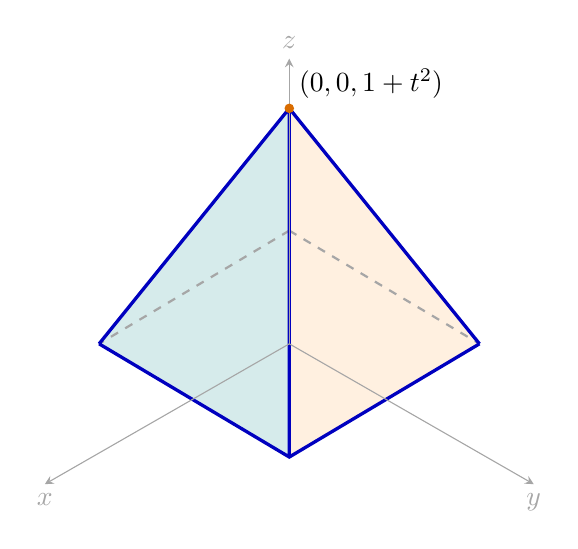
\begin{tikzpicture}[scale=1.15,>=stealth]
    \coordinate (O) at (0,0);
    \coordinate (T) at (0,2.6);
    \coordinate (N) at (0,1.25);
    \coordinate (E) at (2.1,0);
    \coordinate (S) at (0,-1.25);
    \coordinate (W) at (-2.1,0);
    \fill[blue!8] (N)--(E)--(S)--(W)--cycle;
    \fill[teal!16] (T)--(W)--(S)--cycle;
    \fill[orange!12] (T)--(S)--(E)--cycle;
    \draw[dashed,gray!70,thick] (N)--(E) (N)--(W) (T)--(N);
    \draw[blue!75!black,very thick] (W)--(S)--(E) (T)--(W) (T)--(S) (T)--(E);
    \draw[->,gray!70] (O)--(-2.7,-1.55) node[below] {$x$};
    \draw[->,gray!70] (O)--(2.7,-1.55) node[below] {$y$};
    \draw[->,gray!70] (O)--(0,3.15) node[above] {$z$};
    \fill[orange!85!black] (T) circle (1.5pt);
    \node[above right] at (T) {$(0,0,1+t^2)$};
  \end{tikzpicture}
  \caption{4枚の接平面と $xy$ 平面で囲まれる四角錐}
\end{figure}

\paragraph{(1)}

$V(t) = \dfrac{1}{3} \cdot (t^2+1) \cdot \dfrac{(t^2+1)^2}{t^2} = \dfrac{1}{3} \dfrac{1}{t^2} (t^2+1)^3$

\paragraph{(2)}

$V(t) > 0$ から ($\because 0 < t < 1$) (1)の両辺自然対数をとって，微分して
\begin{align}
  \log V(t) &= -\log 3 + 3 \log(t^2+1) - 2 \log t \\
  \dfrac{V'(t)}{V(t)} &= \dfrac{6t}{t^2+1} - \dfrac{2}{t} = \dfrac{2(2t^2-1)}{t(t^2+1)}
\end{align}
$V(t) > 0$から 増減表をえる
\begin{center}
  \begin{table}[htb]
    \centering
    \begin{tabular}{|c|c|c|c|c|c|} \hline
      $t$ & $0$ & $\cdots$ & $\dfrac{\sqrt{2}}{2}$ & $\cdots$ & $1$ \\ \hline
      $V'$ & & $-$ & $0$ & $+$ & \\ \hline
      $V$ & & $\searrow$ & & $\nearrow$ & \\ \hline
    \end{tabular}
  \end{table}
\end{center}
従って，$t = \dfrac{\sqrt{2}}{2}$ の時 $\min V(t) = \dfrac{9}{4}$ をとる．

☆論述がムズカシイ...

\end{document}
